\section{Evaluation Platform}

Traditionally, the storage constraints of embedded platforms have forced an opacity onto embedded networking stacks, making it difficult to add monitoring logic without removing functionality from the stack itself.
The iterative process of altering the networking stack for any sort of parametric study is intractable for more than a few parameters.
Usually, these parameter spaces are explored with the help of a network simulator such as COOJA~\cite{cooja}, OMNET++~\cite{omnet++} or NS2~\cite{ns2}.
While helpful for establishing estimates of how a protocol under a set of parameters might perform, it is difficult to evaluate the practicality of a protocol without having implemented it in a real system.
Using a modern platform with relaxed storage constraints and increased programmability, we demonstrate a novel platform for full-stack network monitoring on real-world WSN deployments.

\subsection{Hardware Platform}

The hardware platform for typically used network evaluations is the TelosB mote (used in \cite{ko2011evaluating} and modeled in COOJA for network simulations).
The TelosB, introduced in 2005~\cite{polastre2005telos},  employs a 16-bit MSP430 microprocessor with 48 KB ROM and 10 KB RAM.
This was ample space 10 years ago, but as the size and complexity of IPv6 standards and routing standards increased, the increased pressure on code space informed a set of compromises in the design of the TinyOS networking stack, our focal operating system.
These compromises and how they affect the our goal of iterative, parameter-driven evaluation are explored in more detail below.

The recently-introduced Storm platform~\cite{andersen2016system} used in this study has a 32-bit ARM Cortex M4, with 512 KB ROM and 64 KB RAM, offering much more processing power and storage capabilities.

\begin{figure}[t]
\centering
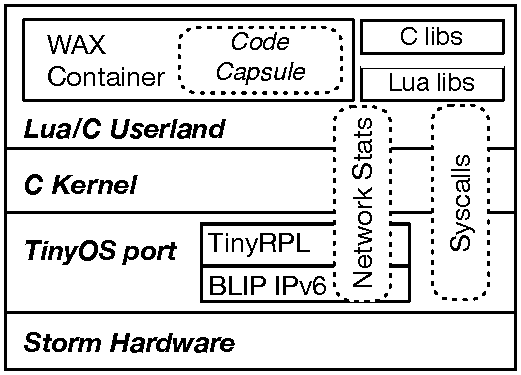
\includegraphics[width=.9\linewidth]{figs/NodeStack}
\caption{The full hardware/software stack for network experimentation. Kernel syscalls take advantage of the synergy between hardware and firmware to expose low-level metrics on the radio
stack that would otherwise be difficult to incorporate.}
\label{fig:nodestack}
\end{figure}


\subsection{Software Platform}

In this section, we discuss the software platform for the Storm motes that are the nodes used in the networking study presented in Section~\ref{section:evaluation}.
The motes run a port of TinyOS 2.x, using the Berkeley Low-Power IPv6 stack (BLIP) and TinyRPL.
Over this, the nodes run the Synergy kernel with a Lua userland~\cite{andersen2016system}, which introduces a dynamic, scripting environment with visibility into the inner workings of the operating system (and thus network stack).
We extend this base functionality with:
\begin{itemize}
\item a set of new syscalls with the ability to edit routing and neighbor tables, and view control traffic and other network telemetry,
\item a network measurement platform Lua library for conducting networking studies
\item a host of tricks for placing two complete routing protocols on a mote with the ability to switch without reflashing
\end{itemize}

Figure~\ref{fig:nodestack} illustrates the full mote platform. \todo{talk about it ocnee the figure is fixed so that WAX is not there}

\subsection{Synergy Kernel and Lua Userland}

\begin{table*}[ht]
\centering
\begin{tabular}{| l | l |}
\hline
\textbf{Syscall} & \textbf{Description} \\ \hline \hline
\multicolumn{2}{|c|}{\texttt{StormSysInfoP.nc}} \\ \hline
\verb`storm.net.retrystats()` & Retrieves transmission and retransmission counts \\ \hline
\verb`storm.net.thopstats()` & Retrieves number of RS and RA with 3hop options sent \\ \hline
\verb`storm.net.rplstats()` & Retrieves number of DIO, DIS and DAO messages sent \\ \hline
\verb`storm.net.stats()` & BLIP-stats: packets sent, forwarded, dropped, fragmented \\ \hline
\multicolumn{2}{|c|}{\texttt{StormRoutingTableP.nc}} \\ \hline
\verb`storm.os.addroute(pfx, len, nhop, iface)` & Add route via nexthop over given interface to routing table \\ \hline
\verb`storm.os.delroute(routekey)` & Removes given route from routing table \\ \hline
\verb`storm.os.lookuproute(pfx, pfx)` & Returns routing table entry matching the given prefix, length \\ \hline
\verb`storm.os.gettable()` & Returns all valid entries in the routing table \\ \hline
\verb`storm.os.flushroutes()` & Deletes all entries from the routing table \\ \hline
\verb`storm.os.flushneighbors()` & Deletes all entries from neighbor table \\ \hline

\end{tabular}
\caption{List of new syscalls implemented for stack monitoring. Each of the \texttt{stats()} methods has a corresponding \texttt{clear()} to erase the cumulative counts.}
\label{table:syscalls}
\end{table*}

A detailed study of a layer 3 routing protocol, such as RPL, needs to be able to pull information from layer 2 and layer 1 components in the networking stack.
The Synergy kernel exposes TinyOS functionality to userland applications through the use of syscalls, giving applications the ability to run timers, send or receive network traffic, and write to GPIO pins or other peripherals.
These syscalls are supported within TinyOS by a set of drivers, which are special TinyOS components.
We add two additional drivers: \texttt{StormRoutingTableP.nc}, which lets applications view and edit the routing and neighbor tables in BLIP; and \texttt{StormSysInfoP.nc}, which exposes routing state, packet counts, retry counts and routing control traffic counts, among other statistics.
A list of the added syscalls can be found in Table~\ref{table:syscalls}.

(Embedded) Lua~\cite{elua} is an embeddable, lightweight, stack-based, high-level scripting language that is easily extensible in C.
Because Lua is an interpreted language, we can add new code at runtime in the form of \emph{code capsules} which we disseminate through a network.
Deployed applications can get large (1800 bytes for a simple traffic generation program) compared to 802.15.4 frames, which are only 127 bytes, predicating the need for a code reassembly mechanism.
The mechanism for dynamically adding logic to a running mote is enabled through a C function that accepts string buffers that contain segments of code.
We deliver code over TCP, using a recent adaptation of the BSD TCP stack to TinyOS.
Each mote listens on a known port for incoming code segments, and hands them to the built-in Lua-C API function \texttt{LuaL\_loadbuffer}, which attempts to evaluate the buffer as a chunk of Lua code.
If the chunk is ``complete'' --- that is, a syntactically valid piece of Lua code --- then it is executed, the results are placed on the Lua stack and interpreted, and the buffer is emptied.
Out-of-memory errors can occur if a buffer forms a large Lua code segment that is not terminated (such as within a large \texttt{while} statement).
It is difficult to recover from out-of-memory errors on an embedded platform; this encourages the dissemination of small, modular functions or tuning variables for preloaded applications.

A limitation of the current version of dynamic code loading is that the code is saved to RAM, which is lost on reboot.
This places limits on what code must be placed on the mote before deployment and what code can be dynamically loaded over the network after the mote is deployed.
Broadly, these constraints force low-level routing protocol code to be programmed into the ROM (not lost on reboot) of each mote, along with the methods handling code reassembly and the basic methods for the network measurement platform described below.
Custom telemetry methods and experiment execution scripts can be loaded dynamically over the network.

Traditionally, switching between routing protocol implementations has required reprogramming (``reflashing'') each individual mote, which is a lengthy and manual process that quickly becomes tedious at even modest numbers of motes.
As discussed below, currently the only way to determine which routing protocol should be run is to check at boot for some flag and determine which routing protocol to start.
While conceivably one could ``stop''\footnote{Using TinyOS's \texttt{StdControl} interface, which provides both \texttt{.start()} and \texttt{.stop()} methods} one routing protocol and switch to another without rebooting, this would also require stopping and cancelling the family of timers and triggers required by the previously running routing protocol.

\subsection{Network Measurement Platform}

Each network experiment comprises five elements: initialization, start condition, traffic generation, stop condition, reporting.
Our network measurement platform provides default methods for each of these elements, which can be strung together using scripting code sent over the network.
New methods and data structures can also be disseminated 

\if 0
Introduce the software stack we're working with:
- 
\fi

%The storage constraints of the older platforms on which BLIP and TinyRPL were developed led to the use of compile-time configuration options (e.g. %\verb`#define` and \verb`#ifdef`) to remove unused features from the compiled stack when flashing motes.
%Although the Storm platform does not possess the same storage constraints, the status of the current codebase limits the %ability to use userland applications to configure the TinyOS networking stack.
%Refactoring the codebase to use run-time rather than compile-time parameters is a not insignificant task, but the WAX methodology could be easily extended to pass configuration options to the TinyOS networking stack to change the choice of objective function or other RPL parameters.

\if 0
talk about tinyos? blip?

Many recent features of  ipv6 nd not implemented
many constants vital to the protocol buried deep in header files with #define so that they
  can be placed into more plentiful ROM. Can't be edited at runtime
\fi

\if 0
- many prior measurements done exclusively on simulators
    - few experiments run in the real world
    - if using a Java implementation, can totally put in all features you want and
      easy to chagne parameters, but this doesn't help us evaluate how well protocol works
- Hardware:
    - advancements in hardware make


- establish the measurement apparatus for these:
    - TinyOS Kernel
    - Syscalls in Lua
        - challenges developing syscalls
    - Dynamic code loading in Lua
    - fitting everything into the mote
        - memory issues
        -  trigger issues: receive a rogue message can mess everything up because function is still there and wired up!
    - "WAX stack"
        - follow similar structure to the sensys paper
        - the components of a network experiment code
        - how to we do logging, where it goes
\fi
